\documentclass[a4paper]{scrartcl}

\usepackage[ngerman]{babel}
\usepackage[utf8]{inputenc}
\usepackage[T1]{fontenc}
\usepackage{graphicx}
\usepackage{tabularx}
\usepackage{enumitem}

\title{Compi-Flick: Use-Cases}
\author{Damien Flury}
\date{9. September 2020}

\begin{document}
\maketitle
\begin{figure}
  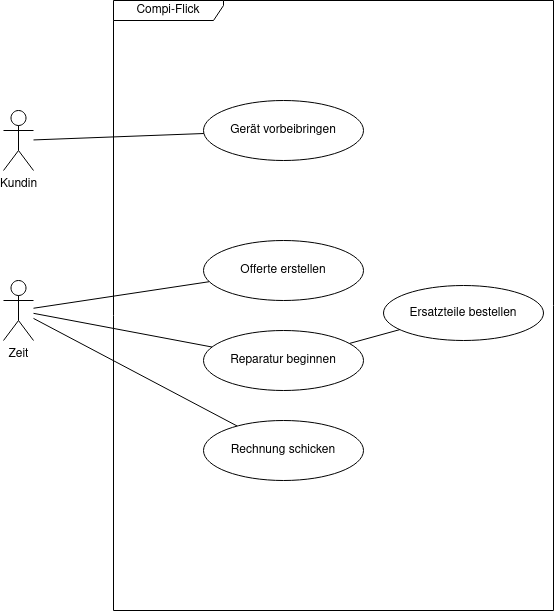
\includegraphics[width=\textwidth]{images/compi-flick-use-case.png}
  \caption{Use-Case-Diagramm}
\end{figure}

\section{Use Cases}
\subsection{Gerät vorbeibringen}
\begin{tabularx}{\textwidth}{l|X}
  
  Motivation & Dieser Anwendungsfall wird von
  der Kundin ausgelöst. Er ist wichtig, dass eine
  Reparatur starten kann. \\ 
  Auslöserin & Die Kundin \\ 
  Input & Das Gerät und eventuelle Informationen, welche
  die Kundin hat (z.B. Schadenursache) sind Argumente, welche
  die Kundin ans System übergibt. \\ 
  Rate & Einmal pro Reparatur \\ 
  Output &
  \begin{minipage}[t]{\linewidth}
  \begin{itemize}[nosep,after=\strut]
    \item Nachricht an Kundin, dass das Gerät akzeptiert wird.
    \item Offerte an Kundin geben.
    \item Repariertes Gerät an Kundin zurückgeben.
    \item Rechnung an Kundin schicken.
  \end{itemize}
  \end{minipage} \\
  Ablauf & Die Kundin geht in eine Filiale und
  gibt ihr Gerät ab. \\ 
  Reaktionszeit & Die Gesamtdauer mit allen Abhängigkeiten
  dauert die ganze Zeit über, also 3-4 Wochen. Der Use Case selbst
  bis zur ersten Antwort dauert Sekunden bis Minuten. \\
\end{tabularx}

\subsection{Offerte erstellen}
\begin{tabularx}{\textwidth}{l|X}
  Motivation & Hat eine Kundin einmal ein Gerät
  vorbeigebracht, wird dieser Use-Case von der Zeit
  ausgelöst. Er ist wichtig, dass die Kundin ungefähre
  Kosten kennt. \\ 
  Auslöserin & Die Zeit \\ 
  Input & Die Daten des analysierten Gerätes dienen
  als Input. \\ 
  Rate & Einmal pro Reparatur \\ 
  Output & Die Offerte wird an Kundin geschickt. \\
  Ablauf & Eine Mitarbeiterin erstellt eine Offerte,
  welche für die Reparatur des Gerätes ungefähr passt. \\
  Reaktionszeit & Stunden bis Tage \\
\end{tabularx}

\subsection{Gerät reparieren}
\begin{tabularx}{\textwidth}{l|X}
  Motivation & Dieser Anwendungsfall wird ausgelöst,
  damit die eigentliche Arbeit -- die Reparatur des Gerätes --
  stattfinden kann. \\
  Auslöserin & Die Zeit \\
  Input & Das kaputte Gerät \\
  Rate & Normalerweise einmal pro Reparatur. In manchen Fällen
  muss ein Gerät vielleicht durch mehrere Iterationen 
  repariert werden. \\
  Output & Das reparierte Gerät \\
  Ablauf & Eine Mitarbeiterin nimmt das Gerät und
  repariert es. \\
  Reaktionszeit & Tage bis Wochen \\
\end{tabularx}

\end{document}